\chapter{Generalized Spinning Switches}
\label{cha:SpinningSwitches}

In this chapter, we explore puzzles about switches on the corners of a
spinning table. Such puzzles have been written about and generalized since they
were first popularized by Martin Gardner.
In this chapter, we provide perhaps the fullest generalization yet, modeling
both the switches and the spinning table as a wreath product of two arbitrary
finite groups. We classify large families of wreath products depending on
whether or not they correspond to a solvable puzzle, completely resolving the
problem for $p$-groups, and providing novel examples for other families of
groups, including two interchangeable copies of the monster group $M$.
Lastly, we provide a number of open questions and conjectures, and
provide other suggestions of how to generalize some of these ideas further.

\section{Overview and preliminaries}
\label{sec:overviewAndPreliminaries}
The paper is organized into six sections.
This section,
Section \ref{sec:overviewAndPreliminaries} provides a brief history of this genre of puzzles and introduces some of the first approaches to generalizing the puzzle further.
Section \ref{sec:WreathModel} models these generalizations in the context of the wreath product, and formalizes the notation of puzzles being solvable.
Section \ref{sec:Reductions} explores situations where the puzzle does not have a winning strategy, and provides reductions that allow us to prove that entire families of puzzles are not solvable.
Section \ref{sec:pGroupStrategy} constructs a strategy for switches that behave like $p$-groups, and gives us ways of building strategies from smaller parts.
Section \ref{sec:OtherSwitchingStrategies} provides novel examples of puzzles that do not behave like $p$-groups, but still have winning strategies.
Lastly,
Section \ref{sec:OpenQuestions} provides further generalizations, and contains dozens of conjectures, open questions, and further directions.

\subsection{History}
Spinning Switches puzzles are a family of closely related puzzles
that were first popularized by Martin Gardner in the form of pint glasses
on a lazy susan.
In the February 1979 edition of his column ``Mathematical Games.'' \cite{Gardner1979Problem}
Gardner writes that he learned of the puzzle from Robert Tappay of Toronto who
``believes it comes from the U.S.S.R.,'' a history that is not especially
forthcoming.

My preferred version of the puzzle appears in Peter Winkler's 2004 book
\textit{Mathematical Puzzles A Connoisseur's Collection}
\begin{quote}
  Four identical, unlabeled switches are wired in series to a light bulb.
  The switches are simple buttons whose state cannot be directly observed,
  but can be changed by pushing; they are mounted on the corners of a
  rotatable square. At any point, you may push, simultaneously, any subset
  of the buttons, but then an adversary spins the square. Show that there
  is a deterministic algorithm that will enable you to turn on the bulb in
  at most some fixed number of steps. \cite{Winkler2004}
\end{quote}

(Winkler's version will be a working example in many parts of the paper, so it
is worth keeping in mind.
An illustration can be found in Figure \ref{fig:twoSwitches}.)

Over the last three decades, various authors have consider generalizations of
this puzzle. Here, we build on those results and go further.
The first place authors looked to generalize was suggested by Gardner himself.
In his March 1979 column, he provided the answer to the original puzzle and wrote
\begin{quote}
The problem can also be generalized by replacing glasses with objects that
have more than two positions. Hence the rotating table leads into deep
combinatorial questions that as far as I know have not yet been explored.
\cite{Gardner1979Solution}
\end{quote}

In 1993, Bar Yehuda, Etzion, and Moran \cite{BarYehuda1993}. took on the challenge and developed a theory
of the spinning switches puzzle where the switches behave like roulettes
with a single ``on'' state. In this chapter we take Gardner's charge to
it's logical conclusion and consider switches that behave like arbitrary
``objects that have more than two positions''.

Another generalization of this puzzle could look at other ways of ``spinning''
the switches. In 1995, Ehrenborg and Skinner \cite{Ehrenborg1995} did this
in a puzzle they call "Blind Bartender with Boxing Gloves", that analyzed
this puzzle while allowing the adversary to use an arbitrary, faithful group action
to ``scramble'' the switches. We analyze our generalized switches within this
same context.

This puzzle was re-popularized in 2019 when it appeared in ``The Riddler''
column from the publication FiveThirtyEight \cite{FiveThirtyEight}.
Shortly after this, in 2022, Yuri Rabinovich synthesized Bar Yehuda and Ehrenborg's
results in a a paper that modeled the collection of switches as a vector space
over a finite field, and modeled the ``spinning'' or ``scrambling'' as a
faithful, linear group action.

Sidana \cite{Sidana2020} provides a detailed overview of the history of this
and related problems.

\subsection{A solution to Winkler's Spinning Switches puzzle}

We will start by discuss the solution to Winkler's version of the puzzle because
the solution provides some insights and intuition for the techniques that we use
later. Before solving the four-switch version of the puzzle,
we will make Peter Winkler proud by beginning with a simpler, two-switch version.

\begin{example}
  Suppose that we have two identical unlabeled switches on opposite corners
  of a square table, as in Figure \ref{fig:twoSwitches}

  Then we have a three-step solution for solving the problem. We start by
  toggling both switches simultaneously. If this does not turn on the light,
  this means that the switches were (and still) are in different states.

  Then, the adversary spins the table. Next, we toggle one of the two switches
  to ensure that the switches are both in the same state. If the light hasn't
  turned on, both must be in the off state.

  The adversary spins the table once more, but to no avail. We know both
  switches are in the off state, so we toggle them both simultaneously, turning
  on the lightbulb.
\end{example}

\begin{figure}
  \center
  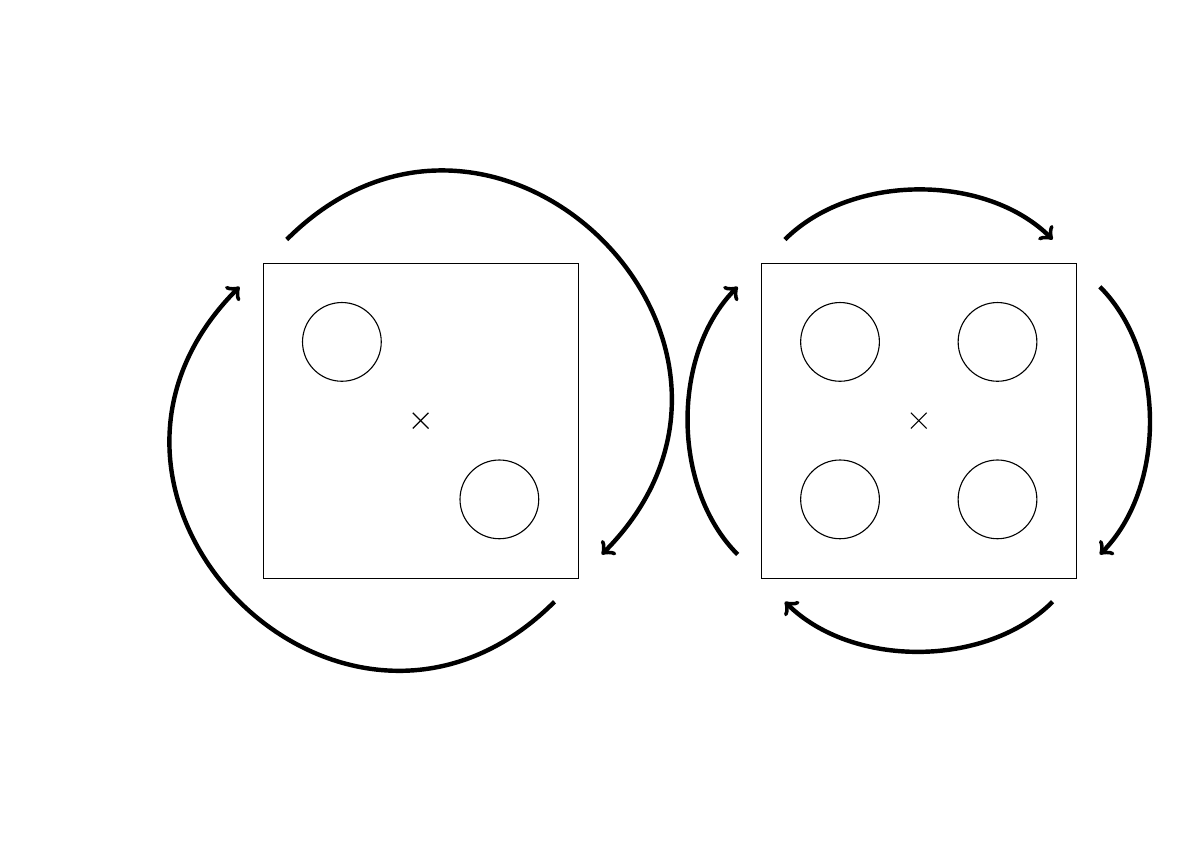
\begin{tikzpicture}
    % Two switches
    % ---------------------
    \draw (0,0) rectangle (4,4);
    \draw (2.1,1.9)--(1.9,2.1);
    \draw (2.1,2.1)--(1.9,1.9);
    \draw (1,3) circle (0.5);
    \draw (3,1) circle (0.5);
    \draw[ultra thick, ->] (0.3, 4.3) to[out=45, looseness=1.7, in=45] (4.3,0.3);
    \draw[ultra thick, ->] (3.7,-0.3) to[out=225, looseness=1.7, in=225] (-0.3, 3.7);

    % Four switches
    % ---------------------
    \draw[xshift=18em] (0,0) rectangle (4,4);
    \draw[xshift=18em] (2.1,1.9)--(1.9,2.1);
    \draw[xshift=18em] (2.1,2.1)--(1.9,1.9);
    \draw[xshift=18em] (1,1) circle (0.5);
    \draw[xshift=18em] (1,3) circle (0.5);
    \draw[xshift=18em] (3,1) circle (0.5);
    \draw[xshift=18em] (3,3) circle (0.5);
    \draw[xshift=18em, ultra thick, ->] (0.3, 4.3) to[out=45, looseness=0.9, in=135] (3.7,4.3);
    \draw[xshift=18em, ultra thick, ->] (4.3,3.7) to[out=-45, looseness=0.9, in=45] (4.3,0.3);
    \draw[xshift=18em, ultra thick, ->] (3.7, -0.3) to[out=-135, looseness=0.9, in=-45] (0.3,-0.3);
    \draw[xshift=18em, ultra thick, ->] (-0.3, 0.3) to[out=-225, looseness=0.9, in=-135] (-0.3,3.7);
  \end{tikzpicture}
  \caption[Illustration of a two-switch and original version of Winkler's ``Spinning Switches''.]{
    Illustration of both the two-switch and Winkler's original four-switch
    version of the puzzle, both on a spinning square table.
  }
  \label{fig:twoSwitches}
\end{figure}

In order to bootstrap the two-switch solution into a four-switch solution,
we must notice two things: \begin{enumerate}
  \item First, if we can get two switches along each diagonal into the same state
  respectively, then we can solve the puzzle by toggling both diagonals
  (all four switches), both switches in a single diagonal, and both diagonals
  again. In this (sub-)strategy, toggling both switches along a diagonal is
  equivalent to toggling a single single switch in the above example.
  \item Second, we can indeed get both diagonals into the same state by toggling a
  switch from each diagonal (two switches on any side of square),
  then a single switch from one diagonal,
  followed by a switch from each switch.
\end{enumerate}

We will interleave these strategies in a particular way, following the notation
of Rabinovich \cite{Rabinovich2022}.

\begin{definition}
  Given two sequences $A = \{a_i\}_{i=1}^N$ and $B = \{b_i\}_{i=1}^M$, we can
  define the \textbf{interleave} operation as \begin{align}
    A \circledast B &= (A,b_1,A,b_2,A,\dots,b_M,A) \\
      &= (
      \underbrace{a_1, a_2, \dots, a_N}_A,
      b_1,
      \underbrace{a_1, a_2, \dots, a_N}_A,
      b_2,
      \underbrace{a_1, a_2, \dots, a_N}_A,
      \dots,
      b_M,
      \underbrace{a_1, a_2, \dots, a_N}_A).
  \end{align} which has length $(M+1)N + M = MN + M + N$.
\end{definition}

Typically it is useful to interleave two strategies when
$A$ solves the puzzle given that the switches are in a particular state, and
$B$ gets the switches into that particular state.
Usually, we also need $A$ not to ``interrupt'' what $B$ is doing.
In the problem of four switches on a square table,
$B$ will ensure that the switches are in the same state within each diagonal,
and $A$ will turn on the light when that's the case.
Moreover, $A$ does not change the state within each diagonal.

\begin{proposition}
  There exists a fifteen-move strategy that guarantees that the light in
  Winkler's puzzle turns on.
  \label{prop:WinklersSolution}
\end{proposition}
\begin{proof}
  We begin by formalizing the two strategies. We will say that the first
  strategy $S_1$ where we toggle the two switches in a diagonal together
  will consist of the following three moves: \begin{enumerate}
    \item Switch \textbf{a}ll of the bulbs ($A$).
    \item Switch the \textbf{d}iagonal consisting of the upper-left and lower-right bulbs ($D$).
    \item Switch \textbf{a}ll of the bulbs ($A$).
  \end{enumerate}
  We will say that the second strategy $S_2$ where we get the two switches
  within each diagonal into the same state consists of the following three
  moves: \begin{enumerate}
    \item Switch both switches on the left \textbf{s}ide ($S$).
    \item Switch \textbf{one} switch ($1$).
    \item Switch both switches on the left \textbf{s}ide ($S$).
  \end{enumerate}
  Then the $15$ move strategy is \[
    S_1 \circledast S_2 = (A, S, A, D, A, S, A, 1, A, S, A, D, A, S, A)
  \]
\end{proof}

We will generalize this construct in
Theorem \ref{thm:switchingStrategyDecomposition},
which offers a formal proof that this strategy works.

It is worth briefly noting that $S_1 \circledast S_2$ is the fourth
\textit{Zimin word} (also called a \textit{sequipower}),
an idea that comes up in the study of combinatorics on words.

\subsection{Generalizing switches}
\label{sec:GeneralizingSwitches}
Two kinds of switches are considered by Bar Yehuda, Etzion, and Moran in 1993
\cite{BarYehuda1993}: switches with a single ``on'' position that behave like
$n$-state roulettes ($\mathbb Z_n$) and switches that behave like
the finite field $\mathbb F_q$, both on a rotating $k$-gonal table.
Yuri Rabinovich \cite{Rabinovich2022} goes further by considering collections
of switches that behave like arbitrary finite dimensional vector spaces over
finite fields that are acted on by a linear, faithful group action.
We generalize this notion further by considering switches that behave like
arbitrary finite groups.

\begin{example}
In Figure \ref{fig:S3Switch}, we provide a schematic for a switch that behaves
like the symmetric group $S_3$.
It consists of three identical-looking parts that need to be
arranged in a particular order in order for the switch to be on.

We could also construct a switch that behaves like the dihedral group of the
square, $D_8$. This switch a flat, square prism that can slot into a square hole,
and only one of the $|D_8| = 8$ rotations of the prism completes the circuit.
\label{ex:S3D8Schematics}
\end{example}

\begin{figure}
  \center{
  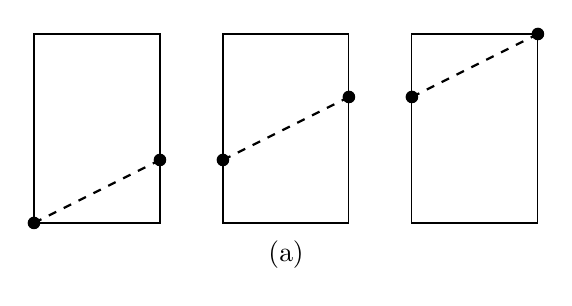
\begin{tikzpicture}[scale=0.8]
    \draw (0,0) rectangle ++(2,3);
    \draw[dashed,thick] (0,0) -- ++(2,1);
    \fill (0,0) circle (0.1);
    \fill (2,1) circle (0.1);

    \draw (3,0) rectangle ++(2,3);
    \draw[dashed,thick] (3,1) -- ++(2,1);
    \fill (3,1) circle (0.1);
    \fill (5,2) circle (0.1);

    \draw (6,0) rectangle ++(2,3);
    \draw[dashed,thick] (6,2) -- ++(2,1);
    \fill (6,2) circle (0.1);
    \fill (8,3) circle (0.1);
    \node at (4, -1/2) {(a)};
  \end{tikzpicture}
  }

  \noindent
  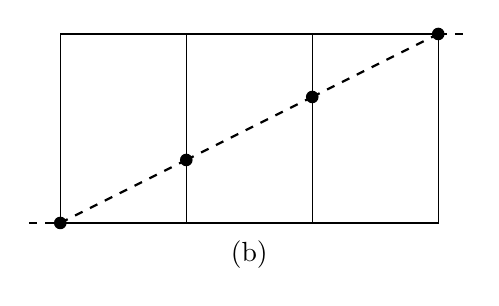
\begin{tikzpicture}[scale=0.8]
    \draw[dashed,thick] (-0.5,0) -- (0,0);
    \fill (0,0) circle (0.1);

    \draw (0,0) rectangle ++(2,3);
    \draw[dashed,thick] (0,0) -- ++(2,1);
    \fill (2,1) circle (0.1);

    \draw (2,0) rectangle ++(2,3);
    \draw[dashed,thick] (2,1) -- ++(2,1);
    \fill (4,2) circle (0.1);

    \draw (4,0) rectangle ++(2,3);
    \draw[dashed,thick] (4,2) -- ++(2,1);
    \fill (6,3) circle (0.1);

    \draw[dashed,thick] (6,3) -- (6.5,3);
    \node at (3, -1/2) {(b)};
  \end{tikzpicture}
  ~
  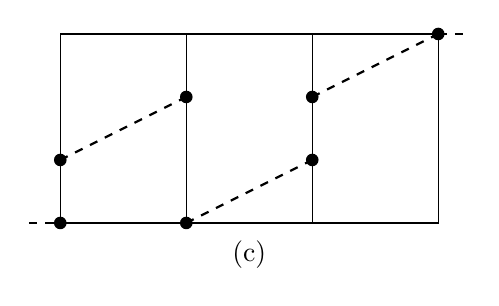
\begin{tikzpicture}[scale=0.8]
    \draw[dashed,thick] (-0.5,0) -- (0,0);
    \fill (0,0) circle (0.1);

    \draw (0,0) rectangle ++(2,3);
    \draw[dashed,thick] (0,1) -- ++(2,1);
    \fill (0,1) circle (0.1);
    \fill (2,2) circle (0.1);

    \draw (2,0) rectangle ++(2,3);
    \draw[dashed,thick] (2,0) -- ++(2,1);
    \fill (2,0) circle (0.1);
    \fill (4,1) circle (0.1);

    \draw (4,0) rectangle ++(2,3);
    \draw[dashed,thick] (4,2) -- ++(2,1);
    \fill (4,2) circle (0.1);
    \fill (6,3) circle (0.1);

    \draw[dashed,thick] (6,3) -- (6.5,3);
    \node at (3, -1/2) {(c)};
  \end{tikzpicture}
  \caption[A schematic for a switch that behaves like $S_3$.]{
    Part (a) shows a simple schematic for the components of a switch that
    behaves like $S_3$, the symmetric group on three letters.
    The three rectangles can be permuted arbitrarily, but only configuration (b)
    completes the circuit. All other configurations fail to
    complete the circuit (e.g., (c)).
  }
  \label{fig:S3Switch}
\end{figure}


One subtlety of using a group $G$ to model a switch is that
both the ``internal state'' of a switch itself and
the set of ``moves'' or changes are modeled by $G$.
Perhaps we think of the state as the underlying set of $G$
and the moves act via right group action of $G$ on itself.

The reason that using a group to model a switch is because groups have many
of the properties we would expect in a desirable switch.
\begin{note}
  The axioms for a group $(G, \cdot)$ closely follow what we would expect from
  a switch.
\end{note}
 \begin{enumerate}
  \item (Closure) The group $(G, \cdot)$ is equipped with a binary operation,
  $\cdot \colon G \times G \rightarrow G$. That is, for all pairs of elements
   $g_1, g_2 \in G$ their product is in $G$ \[
     g_1 \cdot g_2 \in G.
  \]
  In the context of switches, this
  means that if the switch is in some state $g_1 \in G$ and player B moves
  it with action $g_2 \in G$, then $g_1 \cdot g_2 \in G$ is a valid switch for
  the state.
  %
  %
  \item (Identity) There exists an element $\operatorname{id}_G \in G$ such that
  for all $g \in G$, \[
    \operatorname{id}_G \cdot g = g \cdot \operatorname{id}_G = g.
  \]
  This axiom is useful because it means that Player B can ``do nothing''
  to a switch and leave it in whatever state it is in.
  Because the identity is a distinguished element in $G$,
  we will also use the convention that
  $\operatorname{id}_G$ is the ``on'' or ``winning'' state for a given switch.
  (It is worth noting that all of the arguments work with small modification
  regardless of which element is designated as the on state.)
  %
  %
  \item (Inverses) For each element $g \in G$ there exists an inverse element
  $g^{-1} \in G$ such that \[
    g \cdot g^{-1} = g^{-1} \cdot g = \operatorname{id}_G.
  \]
  This axiom states that no matter what state a switch is in,
  there is a move that will transition it into the on state.
  %
  %
  \item (Associativity) Given three elements $g_1, g_2, g_3 \in G$,
  \[
    (g_1 \cdot g_2) \cdot g_3 = g_1 \cdot (g_2 \cdot g_3)
  \]
  This is axiom is not strictly necessary for modeling switches,
  but as we will see in a later definition, it gives us a convenient way to
  describe the conditions for a winning strategy.
  (In Subsection \ref{sub:quasigroupSwitches}, we briefly discuss dropping
  the associativity axiom by considering switches that behave like
  quasigroups with identity.)
\end{enumerate}

% In a similar vein, we could construct a switch that behaves like the dihedral
% group of the square. Perhaps the switch is a thin square prism that fits into a
% square slot in such a way that only one orientation of the prism completes the
% circuit. See Figure \ref{fig:D8Switch} for a simple schematic.
% [A schematic for a switch that looks like $D_4$.]
% Or one could imagine a switch that behaves like the dihedral group of the square,
% $D_8$ where the square has a single, unique orientation that completes the circuit.
% Or abstractly, one could think of each switch as an abstract group element,
% where Player B can multiply by anything they like.

\subsection{Generalizing spinning}
We can also consider generalizations of ``spinning'' the switches.
In particular, we will adopt the generalization from
Ehrenborg and Skinner's \cite{Ehrenborg1995} 1995 paper, which use
arbitrary faithful group actions to permute the switches.
In particular, they provide a criterion that determines which group actions
yield a winning strategy in the case of a given number of ``ordinary'' switches
(those that behave like $\mathbb Z_2$).
Rabinovich \cite{Rabinovich2022} stretches these results a bit further and
looks at faithful linear group actions on collections of switches that behave
are modeled as a finite dimensional vector space over a finite field.
We build on this result in the context of more general switches.

\section{A wreath product model}
\label{sec:WreathModel}
Peter Winkler's version of the puzzle consists of four two-way switches on the
corners of a rotating square table.
The behavior of the switches are naturally modeled as $\mathbb Z_2$, and
the rotating table is modeled as the cyclic group $C_4$. We will take the
wreath product of $\mathbb Z_2$ by $C_4$ in order to get a mathematical model
of the generalized spinning switches puzzle.

\subsection{Modeling generalized spinning switches puzzles}
We don't evoke wreath products arbitrarily: we use them because they are the
right abstraction to model a generalized spinning switches puzzle where
$G$ describes the behavior of the switches,
$\Omega$ describes the positions of the switches, and
the action of $H$ on $\Omega$ models the ways the adversary can permute the switches.

\begin{definition}[\cite{Rotman1999}]
  Let $G$ and $H$ be groups,
  let $\Omega$ be a finite $H$-set, and
  let $K = \prod_{\omega \in \Omega} G_\omega$, where $G_\omega \cong G$
  for all $\omega \in \Omega$.
  Then the \textbf{wreath product} of $G$ by $H$ denoted by $G \wr H$,
  is the semidirect product of $K$ by $H$,
  where $H$ acts on $K$ by $h \cdot (d_\omega) = d_{h^{-1}\omega}$ for $g \in H$ and
  $(g_\omega) \in \prod_{\omega \in \Omega} G_\omega$.
  The normal subgroup $K$ of $G \wr H$ is called
  the \textbf{base} of the wreath product.

  The group operation is $(k, h) \cdot (k', h') = (k(h \cdot k'), hh')$
\end{definition}

An element of $(k, h) \in G \wr H$ represents a turn of the game:
The puzzle-solver chooses an element of the base $k \in K$ to indicate
how they want to modify each of their switches
and then their adversary chooses $h \in H$ and acts with $h$ on $\Omega$ to
permute the switches.

\begin{example}
  Consider the setup in the Winkler's version of the puzzle that consists of
  two-way switches ($\mathbb Z_2$) on the corners of a rotating square
  ($C_4 \cong \langle 0^\circ, 90^\circ, 180^\circ, 270^\circ \rangle$).
  The game itself corresponds to the wreath product $\mathbb Z_2 \wr C_4$.
  We will use the convention that the base of the wreath product, $K$ is
  ordered upper-left, upper-right, lower-right, lower-left; the group
  action is specified by degrees in the clockwise direction.

  Consider the following two turns:
  \begin{enumerate}
    \item During the first turn,
    the puzzle-solver toggles the upper-left and lower-right switches, and
    the adversary rotates the table $90^\circ$ clockwise.
    This is represented by the element \[
      ((1,0,1,0), 90^\circ) \in \mathbb Z_2 \wr C_4.
    \]
    \item During the second turn,
    the puzzle-solver toggles the upper-left switch, and
    the adversary rotates the table $90^\circ$ clockwise.
    This is represented by the element \[
      ((1,0,0,0), 180^\circ) \in \mathbb Z_2 \wr C_4.
    \]
  \end{enumerate}
  %
  As illustrated in Figure \ref{fig:WreathProduct},
  the net result of these two turns is the same as
  a single turn where the puzzle-solver toggles the
  upper-left, upper-right, and lower-left
  switches and the adversary rotates the board $270^\circ$ clockwise.

  \begin{figure}
    \center
    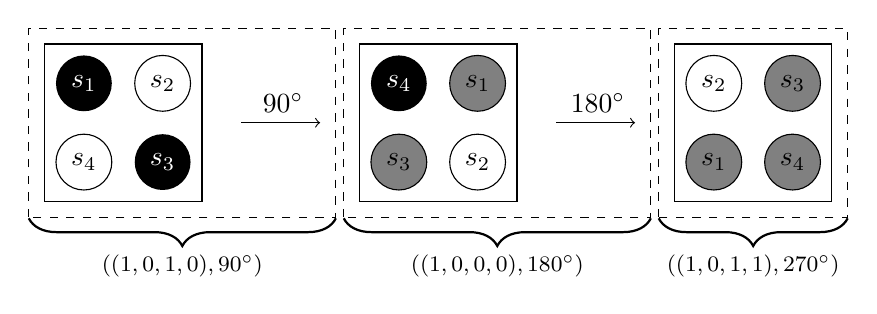
\begin{tikzpicture}
      \draw[dashed] (-0.2,-0.2) rectangle (3.7,2.2);
      \draw [thick,decorate,decoration={brace,amplitude=10pt},yshift=-0.4pt]
        (3.7,-0.2) -- (-0.2,-0.2) node[black,midway,yshift=-0.6cm] {\footnotesize $((1,0,1,0), 90^\circ)$};

      \draw[dashed] (3.8,-0.2) rectangle (7.7,2.2);
      \draw [thick,decorate,decoration={brace,amplitude=10pt},yshift=-0.4pt]
        (7.7,-0.2) -- (3.8,-0.2) node[black,midway,yshift=-0.6cm] {\footnotesize $((1,0,0,0), 180^\circ)$};

      \draw[dashed] (7.8,-0.2) rectangle (10.2,2.2);
      \draw [thick,decorate,decoration={brace,amplitude=10pt},yshift=-0.4pt]
        (10.2,-0.2) -- (7.8,-0.2) node[black,midway,yshift=-0.6cm] {\footnotesize $((1,0,1,1), 270^\circ)$};

      \draw (0,0) rectangle (2,2);
      \node[circle,fill,text=white] at (1/2,3/2) {$s_1$};
      \node[circle,draw] at (3/2,3/2) {$s_2$};
      \node[circle,fill,text=white] at (3/2,1/2) {$s_3$};
      \node[circle,draw] at (1/2,1/2) {$s_4$};
      \draw[->] (2.5,1) -- node[above] {$90^\circ \! \curvearrowright$} (3.5,1) ;

      \draw (4,0) rectangle (6,2);
      \node[circle,fill,text=white] at (9/2,3/2) {$s_4$};
      \node[circle,draw,fill=gray] at (11/2,3/2) {$s_1$};
      \node[circle,draw] at (11/2,1/2) {$s_2$};
      \node[circle,draw,fill=gray] at (9/2,1/2) {$s_3$};

      \draw[->] (6.5,1) -- node[above] {$180^\circ \! \curvearrowright$} (7.5,1) ;

      \draw (8,0) rectangle (10,2);
      \node[circle,draw] at (17/2,3/2) {$s_2$};
      \node[circle,draw,fill=gray] at (19/2,3/2) {$s_3$};
      \node[circle,draw,fill=gray] at (19/2,1/2) {$s_4$};
      \node[circle,draw,fill=gray] at (17/2,1/2) {$s_1$};
    \end{tikzpicture}
    \caption[A wreath product interpretation of a spinning switches puzzle.]{
      An illustration of two turns each in the Spinning Switches puzzle,
      modeled as elements of a wreath product.
    }
    \label{fig:WreathProduct}
  \end{figure}

  The multiplication under the wreath product agrees with this: \begin{align*}
    ((1,0,1,0), 90^\circ) \cdot ((1,0,0,0), 180^\circ)
    &= ((1,0,1,0) + \underbrace{90^\circ \cdot (1,0,0,0)}_{(0,0,0,1)}, 90^\circ + 180^\circ) \\
    &= ((1,0,1,1), 270^\circ)
  \end{align*}
\end{example}

Occasionally it is useful to designate a particular state of the switches as the
``on'' state or the winning state. We will use the convention that the lightbulb
turns on when all of the switches are equal to the identity, that is
$\mathrm{id}_K \in K$.
It is worth noting, however, that the existence of a winning strategy does not
depend on a particular choice in the winning state.
Instead, a winning strategy is equivalent to a choice of moves that will walk
over all of the possible configuration states, regardless of the choice of the
adversaries spin.

\subsection{Switching strategy}

We will begin by formalizing the notation of a winning strategy in a
generalized spinning switches puzzle. Informally, a switching strategy is
a sequence of moves that the puzzle-solver can make that will put the switches
into every possible state, which ensures the the ``on'' state is reached
regardless of the initial (hidden) state of the switches.

\begin{definition}
  A \textbf{switching strategy} for $G \wr H$ is a finite sequence of elements
  in the base $K$,
  $\{k_i \in K\}_{i=1}^N$,
  such that for every sequence of elements in $H$, ${\{h_i \in H\}_{i=1}^N}$,
  \[
    p(\{
      \underbrace{e_{G \wr H}}_{m_0},
      \underbrace{(k_1, h_1)}_{m_1},
      \underbrace{(k_1, h_1)\cdot(k_2, h_2)}_{m_2},
      \cdots,
      \underbrace{(k_1, h_1)\cdot(k_2, h_2)\cdots(k_N, h_N)}_{m_N}
    \}) = K.
  \]
  where $p \colon G \wr H \rightarrow K$ is the projection map from the
  wreath product onto its base.
\label{def:switchingStrategy}
\end{definition}

This definition is useful because it puts the problem into purely algebraic
terms. It is also useful because it abstracts away the initial state of the
switches: regardless of the initial state $k \in K$, a existence of a switching strategy
means that its inverse $k^{-1} \in K$ appears in the sequence.
(This follows the convention that $\mathrm{id}_K \in K$ is designated as the
``on'' state. If $k'$ is chosen to the ``on`` state, then the sequence
must contain $k^{-1}k'$ .)

\begin{proposition}
  A finite sequence of moves is guaranteed to reach the ``on''
  state if and only if it is a switching strategy.
\end{proposition}
\begin{proof}
  Without loss of generality, say that the ``on'' state for the switches is
  $\mathrm{id}_K$.
  In the puzzle, we have an initial (hidden) state, $k$.
  Thus, after the $i$-th move, the wreath product
  element that represents the state of the switches is \[
    p\left((k, \mathrm{id}_H)\cdot(k_1, h_1)\cdot(k_2, h_2)\cdots(k_i, h_i)\right)
    = k \cdot p\left((k_1, h_1)\cdot(k_2, h_2)\cdots(k_i, h_i)\right),
  \] by associativity. We can factor out the first term because
  the ``spin'' is $\mathrm{id}_H$, which acts trivially:
  ${(k, \mathrm{id}_H) \cdot (k', h') = (kk', h')}$

  The initial state can be any $k \in K \setminus \{\mathrm{id}_K\}$,
  and this isn't known to the puzzle-solver.
  In order to reach the ``on'' state, there must exist some $i$, such that
  $p\left((k_1, h_1)\cdot(k_2, h_2)\cdots(k_i, h_i)\right) = k^{-1}$.
  $k$ and adversarial sequences $\{h_i\}_{i=1}^N$.
\end{proof}

It's also worth noting that this model can be thought of as a random model or an
adversarial model: the sequence $\{h_i \in H\}$ can be chosen after the sequence
$\{k_i \in K\}$ in a deterministic way or randomly.

\subsection{Bounds on the length of switching strategies}

One useful consequence of this definition is that it quite straightforward to
prove certain propositions. For example, the minimum length for a switching strategy
has a simple lower bound.
\begin{proposition}
  Every switching strategy $\{k_i \in K\}_{i=1}^{N}$ is a sequence of
  length at least ${|K| - 1}$.
\end{proposition}
\begin{proof}
  This follows from an application of the Pigeonhole Principle. Because the set \[
    \{e_{G \wr H}, (k_1, h_1), (k_1, h_1)\cdot(k_2, h_2), \cdots, (k_1, h_1)\cdot(k_2, h_2)\cdots(k_N, h_N)\}
  \] has at most $N+1$ elements. In order for the projection to be equal to $K$, \[
    p(\{e_{G \wr H}, (k_1, h_1), (k_1, h_1)\cdot(k_2, h_2), \cdots, (k_1, h_1)\cdot(k_2, h_2)\cdots(k_N, h_N)\}) = K,
  \] it must be the case that $N+1 \geq |K|$. Therefore $N \geq |K| - 1$.
\end{proof}

Minimal length switching strategies are common, so we give them a name.
\begin{definition}
  A \textbf{minimal switching strategy} for $G \wr H$ is a switching strategy
  of length $N = |K| - 1.$
\end{definition}

In practice, every wreath product known by the author to have a switching
strategy also has a known minimal switching strategy.
In Section \ref{sec:OpenQuestions}, we ask whether this property always holds.

% 2DO: uncomment and fix this section.
% \subsection{Upper bound for the length of switching strategies}
% Of course, switching strategies can be arbitrarily long.
% For instance, adding any prefix or suffix to a switching strategy again
% results in a switching strategy. However, given a long switching strategy, we
% may want to be able to detect when a shorter one exists.

% We begin with an example that illustrates how this works.

% \begin{proposition}
%   Whenever $G \wr H$ has a switching strategy, it also has a switching strategy
%   of length $N < 2^{|K/H|-1}$, where $K/H$ is the set of equivalence classes of
%   $K$, where $k \sim k'$ if $k = k'h$ for some $h \in H$.
% \end{proposition}

% \begin{proof}
%   % (?) Nondeterministic finite automaton? (?)
%   % Let $K$ act on an element $[k'] \in K/H$ by
%   % $[k']\cdot k = \{[k'(h\cdot k)] : h \in H\}$.
% \end{proof}

\section{Reductions}
\label{sec:Reductions}
In this section, we develop examples of generalized spinning switches puzzles
that do not have switching strategies using three techniques:
directly, by a reduction on switches, or by a reduction on spinning.
%
\subsection{Puzzles known to have no switching strategies}
Our richest collection of known puzzles without switching strategies comes from
a theorem of Rabinovich, which models switches as a vector space over
a finite field.
\begin{theorem} \cite{Rabinovich2022}
  Assume that a finite ``spinning'' group $H$ acts linearly and faithfully on
  a collection of switches that behave like a vector space
  $V$ over a finite field $\mathbb F_q$ of characteristic $p$.
  Then the resulting puzzle has a switching strategy if and only if $H$ is a
  $p$-group.
  \label{thm:Rabinovich}
\end{theorem}
It's worth noting that Rabinovich's switches are less general than arbitrary
finite groups, but the ``spinning'' is more general: in addition to permuting
the switches, the group action might add linear combinations of them as well.
\begin{example}
  By the theorem of Rabinovich \cite{Rabinovich2022},
  the game $\mathbb Z_2 \wr C_3$ does not have a
  switching strategy. In Rabinovich's notation, the vector space of switches
  is $\mathbb Z_2^3$ over the field $\mathbb F_2 = \mathbb Z_2$.
  \label{ex:NoSolutionZ2C3}
\end{example}

The wreath product $\mathbb Z_2 \wr C_3$ is perhaps the simplest example of a
generalized spinning switches puzzle without a switching strategy,
so we will continue to use it as a basis of future examples.

\subsection{Reductions on switches}
With Theorem \ref{thm:Rabinovich} providing a family of wreath products without
spinning switches to reduce to, we now introduce a theorem that allows us to
prove that large families of wreath products also do not have a switching
strategy.
\begin{theorem}
  If $G \wr H$ does not have a switching strategy and $G'$ is a group with
  a quotient $G'/N \cong G$, then ${G'} \wr H$ does not have a switching
  strategy.
  \label{thm:SwitchReduction}
\end{theorem}
\begin{proof}
  We will prove the contrapositive, and suppose that $G' \wr H$ has base $K'$
  and a switching strategy $\{k'_i \in K'\}_{i=1}^N$.

  The quotient map
  $\varphi\colon G' \mapsto G$
  extends coordinatewise to
  $\varphi \colon K' \mapsto K$,
  which further extends in the first coordinate to $G \wr H$:
  $\varphi(k,h) := (\varphi(k), h)$.

  It is necessary to verify that $\varphi\colon G' \wr H \rightarrow G \wr H$
  is indeed a homomorphism.
  \begin{align*}
    \varphi((k'_\alpha, h_\alpha)) \cdot \varphi((k'_\beta, h_\beta))
    &= (\varphi(k'_\alpha), h_\alpha) \cdot (\varphi(k'_\beta), h_\beta) \\
    &= (\varphi(k'_\alpha)(h_\alpha\cdot\varphi(k'_\beta)), h_\alpha h_\beta) \\
    &= (\varphi(k'_\alpha)\varphi(h_\alpha\cdot k'_\beta), h_\alpha h_\beta) \\
    &= (\varphi(k'_\alpha(h_\alpha\cdot k'_\beta)), h_\alpha h_\beta) \\
    &= \varphi((k'_\alpha(h_\alpha\cdot k'_\beta), h_\alpha h_\beta)) \\
    &= \varphi((k'_\alpha, h_\alpha) \cdot (k'_\beta, h_\beta))
  \end{align*}

  Therefore the sequence $\{\varphi(k'_i) \in K\}_{i=1}^N$ is a
  switching strategy on $G \wr H$, because the quotient map
  $\varphi \colon G' \rightarrow G$
  (and thus $\varphi \colon K' \rightarrow K$)
  is injective.
\end{proof}
\begin{example}
  We know that $\mathbb Z_2 \wr C_3$ doesn't have a switching strategy.
  This means that $\mathbb Z_6 \wr C_3$ does not have a switching strategy either,
  as illustrated in Figure \ref{fig:Z2C3}.
  \begin{figure}
    \center
    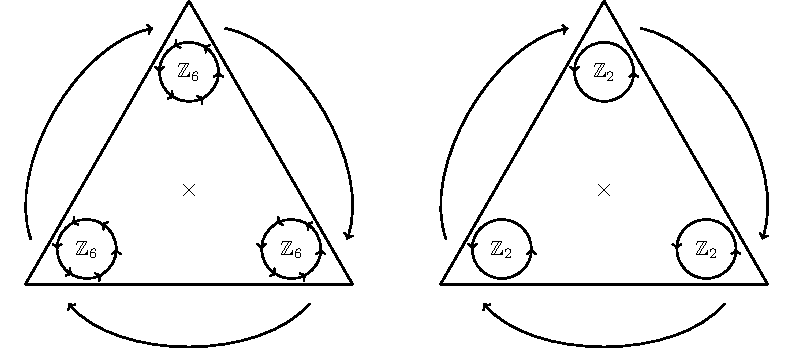
\includegraphics{assets/tikz_Z2C3.pdf}
    \caption[A reduction from a six-way switch to a two-way switch]{
      A reduction on switches:
      $\mathbb Z_6 \wr C_3$ reduces to $\mathbb Z_2 \wr C_3$,
      which is known not to have a switching strategy.
    }
    \label{fig:Z2C3}
  \end{figure}
\end{example}
\subsection{Reductions on spinning}
We can do two similar reductions on the ``spinning'' group of a wreath product.
These theorems say that if a given wreath product $G \wr H$ does not have a
switching strategy, then a similar wreath product $G \wr H'$ with a
``more complicated'' spinning group $H'$ will not have a switching strategy
either.
\begin{theorem}
  If $G \wr H$ does not have a switching strategy and $H'$ is a group with
  a subgroup $A \leq H'$ such that $A \cong H$, then
  $G \wr H'$ does not have a switching strategy.
  \label{thm:SpinReduction}
\end{theorem}
\begin{proof}
  Again we will prove the contrapositive.
  Assume that $G \wr H'$ does have a switching strategy,
  $\{k_i\}_{i=1}^N$. Then by definition, for any sequence
  $\{h'_i\}_{i=1}^N$, the projection of the sequence \[
    p(\{(k_1, h'_1)\cdot(k_2, h'_2)\cdots(k_i, h'_i)\}_{i=1}^N) = K,
  \] and in particular this is true when $h'_i$ is restricted to be in the
  subgroup $H$. Thus a switching strategy for $G \wr H'$ is also a valid
  switching strategy for $G \wr H$.
\end{proof}

\begin{example}
  Consider the wreath product $\mathbb Z_2 \wr_{\Omega_6} C_3$ where
  $\Omega'$ consists of six switches on the corners of a hexagon as
  illustrated in Figure \ref{fig:Z2C6}. While the group action of $C_3$ on
  $\Omega'$ is not transitive, we know that $\mathbb Z_2 \wr_{\Omega_6} C_3$ does
  not have a switching strategy, because in particular there is no way to
  ensure that the  top, bottom-right, and bottom-left switches hit every state.

  Since $\mathbb Z_2 \wr_{\Omega_6} C_3$ doesn't have a switching strategy,
  $\mathbb Z_2 \wr_{\Omega_6} C_6$ cannot not have a switching strategy either.
  \begin{figure}
    \center
    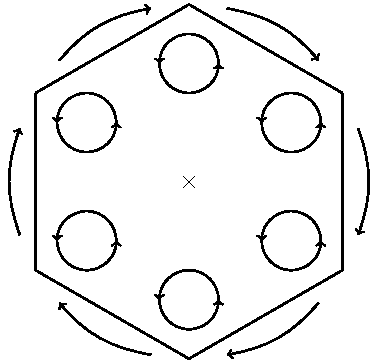
\includegraphics{assets/tikz_Z2C6.pdf}
    \caption{If there were a solution to $\mathbb Z_2 \wr_{\Omega_6} C_6$,
    then there would be a solution to $\mathbb Z_2 \wr_{\Omega_6} C_3$.}
  \end{figure}
  \label{fig:Z2C6}
\end{example}

In the above example, we noted that $\mathbb Z_2 \wr_{\Omega_6} C_3$ does
not have a switching strategy by focusing on a triangle of switches and
using the knowledge that $\mathbb Z_2 \wr C_3$
(two-way switches on a rotating triangular board) does not have a switching
strategy. The following theorem allows us to take that very shortcut.
\begin{theorem}
  Suppose that $H'$ is a group with a subgroup $A \leq H'$ such that
  $A \cong H$,
  and let \[
    \operatorname{Orb}(\omega) = \{\omega \cdot a : a \in A \} \subseteq \Omega
  \]
  be the (right) orbit of $\omega \in \Omega$ under $A$.
  If $G \wr_{\operatorname{Orb}(\omega)} H$ does not have a switching strategy,
  then $G \wr_\Omega H'$ does not have a switching strategy.
  \label{thm:SpinReduction2}
\end{theorem}
\begin{proof}
  We start by making the contrapositive assumption that $G \wr_\Omega H'$
  has a switching strategy ${\{k_i \in K\}_{i=1}^N}$,
  and we consider the projection
  $p_\omega \colon K \rightarrow K_\omega$ where
  \[
    K = \prod_{\omega' \in \Omega} G_{\omega'}
    \hspace{1cm}\text{and}\hspace{1cm}
    K_{\omega} = \prod_{\omega' \in \operatorname{Orb}(\omega)} G_{\omega'}.
  \]

  Then $\{p_\omega(k_i) \in K_\omega\}_{i=1}^N$ is a switching strategy for
  $G \wr_{\operatorname{Orb}(\omega)} H$, since the projection is a surjective
  map.
\end{proof}

\begin{example}
  We know that $\mathbb Z_2 \wr C_3$ doesn't have a switching strategy.
  This means that $\mathbb Z_2 \wr C_6$ does not have a switching strategy either,
  as illustrated in Figure \ref{fig:Z2C6_2}.
\end{example}
\begin{figure}
  \center
  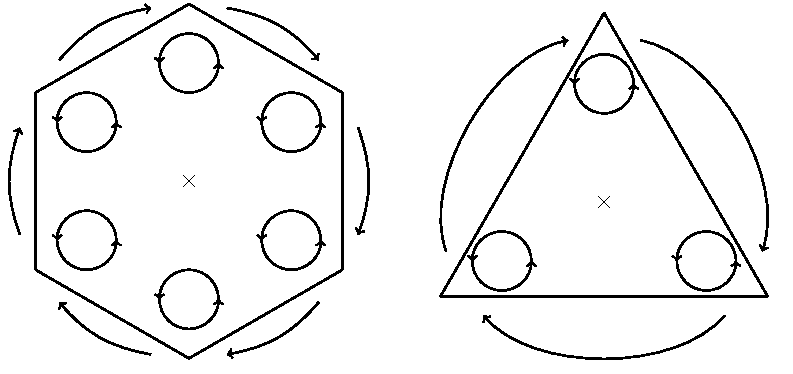
\includegraphics{assets/tikz_Z2C6_2.pdf}
  \caption[A reduction from a hexagonal table to a triangular table.]{
    We know that $\mathbb Z_2 \wr_\Omega C_6$ cannot have
    a switching strategy, because that would imply a switching strategy for
    $\mathbb Z_2 \wr_{\Omega'} C_3$, where $\Omega'$
    is the orbit of the top switch rotations of multiples of $120^\circ$.
  }
  \label{fig:Z2C6_2}
\end{figure}

Now that we've proven that large families of wreath products do not have
switching strategies, it's worthwhile to construct families of wreath products
that do have switching strategies.
%%%%%%%%%%%%%%%%%%%%%%%%%%%%%%%%%%%%%%%%%%%%%%%%%%%%%%%%%%%%%%%%%%%%%%%%%%%%%%
%
% Switching strategies on p-groups
%
%%%%%%%%%%%%%%%%%%%%%%%%%%%%%%%%%%%%%%%%%%%%%%%%%%%%%%%%%%%%%%%%%%%%%%%%%%%%%%
\section{Switching strategies on \texorpdfstring{$p$}{p}-groups}
\label{sec:pGroupStrategy}
In this section, we'll develop a broad family of switching strategies,
namely those where $G$ and $H$ (and thus $G \wr H$) are $p$-groups.
\subsection{Switching strategy decomposition}

Our first constructive theorem provides a technique that can be used to
construct switching strategies for switches that behave like a group $G$ in
terms of a normal group and its corresponding quotient group.
\begin{theorem}
  The wreath product $G \wr H$ has a switching strategy if there exists a
  normal subgroup $N \trianglelefteq G$ such that both $N \wr H$ and
  $G/N \wr H$ have switching strategies.
\label{thm:switchingStrategyDecomposition}
\end{theorem}
\begin{proof}
  Let $S_{G/N} = \{k_i^{G/N} \in K_{G/N}\}$ denote the switching strategy for
  $G/N \wr H$, and
  let $S_{N} = \{k_i^N \in K_{N}\}$ denote the switching strategy for $N \wr H$.

  We ultimately would like to interleave these two strategies,
  but $k_i^{G/N} \not\in K_G$. To find the appropriate analog,
  we partition $G$ into $[G : N] = m$ right cosets of $N$, \[
    G = Ng_1 \sqcup Ng_2 \sqcup \dots \sqcup Ng_m,
  \] each with a chosen representative in $G$.
  Now we define a map $r \colon G/N \rightarrow G$ that chooses the chosen
  representative of the coset, and extends coordinatewise. We use this map to
  define a sequence $S = \{r(k_i^{G/N}) \in K_G\}$.

  We claim that these two sequences interleaved, $S_N \circledast S$, is a
  switching strategy for $G \wr H$. To prove this claim, we observe two facts:
  \begin{enumerate}
    \item Multiplying by elements of $S_N$ will not change cosets and will walk
    through every element of its coset.
    \item Multiplying by elements of $S$ will walk through all cosets.
  \end{enumerate}
  Therefore the interleaved sequence will walk through all elements of each
  coset, and thus is surjective onto $K$.
\end{proof}

\subsection{Construction of switching strategies on \texorpdfstring{$p$}{p}-groups}
We start with a corollary of Theorem \ref{thm:Rabinovich}.
\begin{corollary}
  If $H$ is a finite $p$-group that acts faithfully on $\Omega$,
  then the wreath product
  $G \wr H$ has a switching strategy whenever $|G| = p^n$ for some $n$.
\end{corollary}
\begin{proof}
  A group generated by permutation matrices will act faithfully and linearly on
  a vector space $V$, so it is sufficient to groups $H$ that act faithfully
  by permuting $\Omega$.

  If $|G| = p^n$, then either $G \cong \mathbb{Z}_p$ or $G$ is not simple.

  If $n = 1$, $G \cong \mathbb{Z}_p \cong \mathbb F_p$, then there exists a
  switching strategy by Theorem \ref{thm:Rabinovich}. This is because $H$
  permutes the coordinates of $V = \mathbb F_p^{|\Omega|}$, and so it is a
  linear action on the vector space.

  Otherwise, $G$ is not simple. This means that $G$ has a normal subgroup $N$
  of order $|N| = p^t$ (with $t \geq 1$) and a quotient $G/N$ with order $|G/N| = p^{n-t}$.
  Because $t < n$ and $n - t < n$, we eventually end up at the $n=1$ case by
  induction.
\end{proof}

This means that whenever $G$ and $H$ (and thus $G \wr H$) are $p$-groups,
then $G \wr H$ has a switching strategy.

\subsection{A folklore conjecture}
Here we note a conjecture from folklore, which---if true---implies that we have
\textit{almost} solved the problem in its full generality.
\begin{conjecture}[Folklore]
  Almost all groups are $2$-groups.
\end{conjecture}

One reason for this conjecture is computational. According to the
On-Line Encyclopedia of Integer Sequences \cite{oeis},
there are $A000001(2^{10}) = 49487367289$ groups of order $2^{10}$ and there are
$A063756(2^{11}-1) = 49910536613$ groups of order less than $2^{11}$.
This means that more than $99.15\%$ of the groups of order less than $2^{11}$
are of order $2^{10}$.

If this conjecture is true, then most types of switches have switching
strategies on most kinds of faithful finite group actions.
Of course, while most finite groups may be $2$-groups, most mathematicians
are more interested in groups that \textit{aren't}.
This next section develops two families of examples of switching strategies
where the switches do not behave like $p$-groups.

%%%%%%%%%%%%%%%%%%%%%%%%%%%%%%%%%%%%%%%%%%%%%%%%%%%%%%%%%%%%%%%%%%%%%%%%%%%%%%
%
% Switching strategies on permutations
%
%%%%%%%%%%%%%%%%%%%%%%%%%%%%%%%%%%%%%%%%%%%%%%%%%%%%%%%%%%%%%%%%%%%%%%%%%%%%%%
\section{Switching strategies on other wreath products}
\label{sec:OtherSwitchingStrategies}

Other authors have given switching strategies for various configurations of
generalized spinning switches strategies, but in all of these examples,
the wreath products themselves $p$-groups:
$|G \wr_\Omega H| = |G|^{|\Omega|} \cdot |H|$, where $H$ acts faithfully.
In this section we introduce two families of wreath products that have switching
strategies, but are not $p$-groups.

\subsection{The trivial wreath product, \texorpdfstring{$G \wr \mathbf{1}$}{G wreath trivial group}}
The simplest---and least interesting---way to construct a wreath product with
a switching strategy is to remove the adversary (or randomness) altogether,
by letting the spinning group be the trivial group $H = \mathbf{1}$.
Additionally we will consider the case where $|\Omega| = 1$, so there is only
one switch.
Because the adversary cannot ``spin'' the switches at all, the puzzle-solver has
perfect information the entire time.
We will see that whenever $G$ is a finite group,
$G \wr \mathbf{1} \cong G$ has not just one switching strategy, but many.

\begin{proposition}
  The wreath product $G \wr \mathbf{1}$ has $(|G|-1)!$ minimal switching
  strategies.
  \label{prop:countingTrivialSS}
\end{proposition}
\begin{proof}
  There are $(|G| - 1)!$ permutations of $G \setminus \{\mathrm{id}_G\}$, and
  we claim each one corresponds to a minimal switching strategy. Namely,
  if $(k_1, k_2, \dots, k_{|G|-1})$ is such a permutation, then
  the sequence $\{k'_i\}_{i=1}^{|G|-1}$ where $k'_1 = k_1$ and
  $k'_i = k_{i-1}^{-1}k_i$ is a switching strategy on $G \wr \mathbf{1}$.

  Then we claim by induction that
  $(k'_1, \mathrm{id})\cdot(k'_2, \mathrm{id})\cdots(k'_j, \mathrm{id}) = (k_j, \mathrm{id})$.
  By construction, the base case is true when $j = 1$. If the claim holds up to
  $j-1$, then \[
    \underbrace{
      (k'_1, \mathrm{id})\cdot(k'_2, \mathrm{id})\cdots(k'_{j-1}, \mathrm{id})
    }_{(k_{j-1}, \mathrm{id})}
    (k'_j, \mathrm{id})
    = (k_{j-1}, \mathrm{id})(k_{j-1}^{-1}k_j, \mathrm{id})
    = (k_j, \mathrm{id}),
  \] as desired.
  Thus the projection of the partial products is
  \begin{align}
    &p(\{
      \underbrace{e_{G \wr \mathbf{1}}}_{m_0},
      \underbrace{(k'_1, h_1)}_{m_1},
      \underbrace{(k'_1, h_1)\cdot(k'_2, h_2)}_{m_2},
      \cdots,
      \underbrace{(k'_1, h_1)\cdot(k'_2, h_2)\cdots(k'_N, h_N)}_{m_N}
    \}) \\
    & \hspace{1cm} =
    p(\{
      e_{G \wr \mathbf{1}},
      (k_1, \mathrm{id}),
      (k_2, \mathrm{id}),
      \cdots,
      (k'_N, \mathrm{id})
    \}) \\
    & \hspace{1cm} = \{e_{G \wr \mathbf{1}}, k_1, k_2, \cdots,k_{|G|-1}\} = K,
  \end{align}
  where $\{k_1, k_2, \dots, k_{|G|-1}\}$ spans
  $G \setminus \{\mathrm{id}_G\} \cong K \setminus \{\mathrm{id}_K\}$ by
  assumption.
\end{proof}

While the trivial wreath product is a useful example to keep in mind for
generating counterexamples, we're generally more interested in the situation
where the adversary permutes the switches to create uncertainty for the
puzzle-solver.

\subsection{Two interchangeable groups generated by involutions}

In this section, we will construct a switching strategy for the generalized
spinning switches puzzle that consists of two switches that behave like
a group $G$ that can be generated by involutions, which the adversary can
swap.
(See, for example, Figure \ref{fig:S3Switch} which illustrates switches that
behave like $S_3 = \langle (12), (13)\rangle$)

This strategy relies on the fact that because these generators are their own
inverse, applying a generator to the first switch or the second switch
has no effects on the difference.

This switching strategy has two parts.
The first part ensures that the two switches have every possible difference.
The second part show that we can get the first switch
(with respect to the projection onto $K$)
to take on every possible value without changing the difference.
\begin{theorem}
  Suppose that $G$ is a group that can be generated by involutions.
  Then the generalized spinning switches puzzle consisting of two,
  interchangeable copies of $G$, namely $G \wr C_2$,
  has a switching strategy.
  \label{thm:involutionGeneratedGroups}
\end{theorem}
\begin{proof}
  We start by writing $G$ in terms of its generators:
  $G = \langle t_1, t_2, \dots, t_N \rangle$, where $t_i^{-1} = t_i$.
  Because this is the generating set, there exists a finite sequence of
  transpositions $(t_{i_1}, t_{i_2}, \dots, t_{i_M})$
  such that the partial products of the sequence generate $G$: \[
    G = \{\mathrm{id}_G, t_{i_1}, t_{i_1}t_{i_2}, \dots, t_{i_1}t_{i_2}\cdots t_{i_M}\}.
  \]

  We develop the strategy in two parts. First, we provide a strategy
  $A = \{\alpha_i \in K\}$ such that for any adversarial sequence $\{h_i \in H\}$
  and element $g \in G$, there exists an $i \geq 0$
  such that the {$i$-th} partial product,
  $(g_{i,1}, g_{i,2}) = p((\mathrm{id}_K, \mathrm{id}_H)\cdot(\alpha_1, h_1)\cdot(\alpha_2, h_2)\dots(\alpha_i, h_i))$,
  has a difference of $g$. That is, $g_{i,1}g_{i,2}^{-1} = g$.

  To do this, we define $\alpha_j = (t_{i_j}, \mathrm{id}_G)$,
  and notice that the difference of the coordinates is the same whether we
  add $\alpha_j$ or $(180^\circ)\cdot \alpha_j$ to a element
  $(g_1, g_2) \in K$: \[
    g_1(g_2t_{i_j})^{-1} = g_1t_{i_j}^{-1}g_2^{-1} = (g_1t_{i_j})g_2^{-1}
  \]

  Because the partial products of $t_{i_j}$ cover $G$, there exists some
  $t_1 t_2\dots t_k = g_1{-1}gg^2$, so that $g_{i,1}g_{i,2}^{-1} = g$, as
  desired.

  Next, we give a strategy $B = \{\beta_i\}$ such that for any adversarial
  sequence $\{h_i \in H\}$ and element $g \in G$, there exists an $i \geq 0$
  such that the {$i$-th} partial product,
  $(g_{i,1}, g_{i,2}) = p((\mathrm{id}_K, \mathrm{id}_H)\cdot(\alpha_1, h_1)\cdot(\alpha_2, h_2)\dots(\alpha_i, h_i))$
  has a first coordinate $g_{i,1} = g$.

  To do this, we define $\beta_j = (t_{i_j}, t_{i_j})$. This strategy is
  invariant up to actions of $H$, so we can see that regardless of the initial
  state $(g_1, g_2) \in K$, there exists some $j$ such that
   $\beta_1 \beta_2 \cdots \beta_j = g_1^{-1}g$ and therefore
   $(g_1, g_2) \beta_1 \beta_2 \cdots \beta_j = (g, g_2g_1^{-1}g)$, as desired.

   It is important to note that applying $\beta_j$ does not affect the
   difference: $(g_1, g_2) \beta_j = (g_1t_{i_j}, g_2t_{i_j})$ has a
   difference of
   $(g_1t_{i_j})(g_2t_{i_j})^{-1} = g_1t_{i_j}t_{i_j}^{-1}g_2^{-1} = g_1g_2^{-1}$.

  Now by interleaving these two strategies, we see that the partial products
  of $B \circledast A$ hit every possible first letter and every possible
  difference for every first letter,
  therefore the projection of the partial products of
  $B \circledast A$ cover $K$ for all adversarial sequences, so
  $B \circledast A$ is a switching strategy.
\end{proof}
We will illustrate this idea explicitly letting $G$ be the smallest nonabelian
group of composite order, the symmetric group on three letters $S_3$, which is
isomorphic to the dihedral group of the triangle, $D_6$.
\begin{example}
  Note that $S_3 = \langle(12), (13)\rangle$ is generated by involutions, and
  that the partial products of the sequence $((12),(13),(12),(13),(12))$
  cover $S_3$.

  As a bit of notation, for a permutation $\pi \in S_3$, let
  $\pi_1 = (\pi, \mathrm{id}_{S_3}) \in K$
  and
  $\pi_2 = (\pi, \pi) \in K$, corresponding to sequences $B$ and $A$
  respectively in the above theorem.
  Then the following is a (minimal) switching strategy on $S_3 \wr C_2$:
  \begin{singlespace}
  \begin{align*}
    (12)_2(13)_2(12)_2(13)_2(12)_2 \\
    &(12)_1 \\
    (12)_2(13)_2(12)_2(13)_2(12)_2 \\
    &(13)_1 \\
    (12)_2(13)_2(12)_2(13)_2(12)_2 \\
    &(12)_1 \\
    (12)_2(13)_2(12)_2(13)_2(12)_2 \\
    &(13)_1 \\
    (12)_2(13)_2(12)_2(13)_2(12)_2 \\
    &(12)_1 \\
    (12)_2(13)_2(12)_2(13)_2(12)_2
  \end{align*}
  \end{singlespace}
  \label{ex:TwoSymmetricGroups}
\end{example}
It is natural to ask which generalized spinning switches puzzles with
switches that symmetric groups have switching strategies. We can use a
reduction on switches to rule out a large amount of these.
\begin{proposition}
  For $n > 1$, $S_n \wr H$ does not have a switching strategy whenever
  $|H|$ is not a power of $2$.
\end{proposition}
\begin{proof}
  The alternating group $A_n$ is an index $2$ subgroup of $S_n$, so $A_n$ is
  normal, and $S_n/A_n \cong \mathbb Z_2$.
  Since we know that $\mathbb Z_2 \wr H$ has no switching strategy when
  $|H|$ is not a power of $2$,
  by the reduction in Theorem \ref{thm:SwitchReduction}, $S_n \wr H$ does
  not have a switching strategy.
\end{proof}

Many groups are generated by transpositions, including $22$ of the $26$
sporadic simple groups and the alternating group $A_5$ and $A_n$ for $n > 9$,
as shown by Mazurov and Nuzhin respectively.
\begin{theorem}\cite{Mazurov2003}
  Let $G$ be one of the 26 sporadic simple groups.
  The group $G$ cannot be generated by three involutions two of which commute
  if and only if $G$ is isomorphic to $M_{11}$, $M_{22}$, $M_{23}$, or $M^c_L$.
\end{theorem}
\begin{theorem}\cite{Nuzhin1992}
  The alternating group $A_n$ is generated by three involutions the
  two of which commute, if and only if $n \geq 9$ or $n = 5$.
\end{theorem}

Nuzhin provides other families of groups that are generated by three
involutions, two of which commute, in subsequent papers.
\cite{Nuzhin0,Nuzhin1,Nuzhin2}

Thus, we have characterized finite wreath products with switching strategies
in many cases:
wreath products that are $p$-groups,
trivial wreath products, and
wreath products $G \wr C_2$ where $G$ is generated by involutions.
In the next section, we provide even more general constructions and ask
more specific questions.

%%%%%%%%%%%%%%%%%%%%%%%%%%%%%%%%%%%%%%%%%%%%%%%%%%%%%%%%%%%%%%%%%%%%%%%%%%%%%%
%
% Open questions
%
%%%%%%%%%%%%%%%%%%%%%%%%%%%%%%%%%%%%%%%%%%%%%%%%%%%%%%%%%%%%%%%%%%%%%%%%%%%%%%
\section{Generalizations and open questions}
\label{sec:OpenQuestions}
In this section, we provide conjectures and suggest open questions about
the structure of switching strategies when they exist,
further generalizations of spinning switches puzzles,
and finally introduce a notion of an infinite switching strategy for infinite
wreath products.

The ultimate open question is a full classification
of finite wreath products with switching strategies.
\begin{openquestion}
  What finite wreath products, $G \wr H$, have a switching strategy?
\end{openquestion}
\subsection{Switches generated by elements of prime power order}

In Theorem \ref{thm:involutionGeneratedGroups},
we constructed a strategy for $G \wr C_2$,
when $G$ can be generated by elements of order $2$.
We conjecture that that there is a broader construction for the case where
the adversary can act on the switches with a group of order $2^\ell$.

\begin{conjecture}
  When $G$ is a finite group generated by involutions, and
  $H$ is $2$-group that acts faithfully on the set of switches,
  there exists a switching strategy for $G \wr H$.
\end{conjecture}

We can also ask about three switches that are generated by elements of order
$3$ on the corners of a triangular table. In particular, the alternating group
is such a group, and we conjecture that it has a switching strategy.

\begin{conjecture}
  There exists a switching strategy for $A_n \wr C_3$.
\end{conjecture}

Putting these two conjectures together, we boldly predict a large family
of wreath products with switching strategies.
\begin{conjecture}
  If $G$ can be generated by elements of order $p^n$, and $H$ is a $p$-group
  acting faithfully on the set of switches $\Omega$, then $G \wr_\Omega H$ has
  a switching strategy.
\end{conjecture}

\subsection{Palindromic switching strategies}
In all known examples, when there exists a switching strategy $S$,
we also know of a \textit{palindromic} switching strategy
$S' = \{k'_i \in K\}_{i=1}^N$
such that $k'_i = k'_{N-i+1}$ for all $i$.

\begin{conjecture}
  Whenever $G \wr H$ has a switching strategy, it also has a palindromic switching
  strategy.
\end{conjecture}

If this conjecture is false, we suspect a counterexample can be found in the
case of the trivial wreath product, $G \wr \mathrm{1} \equiv G$.

\subsection{Quasigroup switches}
\label{sub:quasigroupSwitches}
In Section \ref{sec:GeneralizingSwitches}, we argued for modeling switches as
finite groups because of some desirable properties: \begin{enumerate}
  \item Closure. Regardless of which state a switch is in, modifying the state is the set of states.
  \item Identity. We don't have to toggle a switch on a given turn.
  \item Inverses. If a switch is off, we can always turn it on.
\end{enumerate}

In the list, we also included the axiom of associativity for three reasons:
switches in practice typically have associativity,
groups are easier to model than quasigroups with identity, and
it makes the definition of a ``switching strategy'' less fussy.

However, one could design a switch that does not have associativity
because, and the puzzle would still be coherent. This is because the process of
a generalized spinning switches puzzle is naturally
``left associative'' in the language programming language theory:
we are always ``stacking'' our next move onto the right.
As such, it is worth noting the slightly more general way of modeling switches:
as quasigroups with identity, called \textit{loops}.

In particular, we are interested in the smallest loop that is not a group
\cite{MSELoop}, which we denote
$\mathcal{L} = (\{1, a, b, c, d\}, \ast)$,
and describe via its multiplication table, a Latin square of order $5$.
(Notice that $(ab)d = a \neq d = a(bd)$.)
\begin{singlespace}
\[
  \begin{array}{c|ccccc}
    \ast & 1 & a & b & c & d \\
    \hline
      1 & 1 & a & b & c & d \\
      a & a & 1 & c & d & b \\
      b & b & d & 1 & a & c \\
      c & c & b & d & 1 & a \\
      d & d & c & a & b & 1
  \end{array}
\]
\end{singlespace}

\begin{conjecture}
  There exists a nontrivial adversarial group $H$ such that the generalized
  spinning switches puzzle with switches that look like $\mathcal{L}$ has
  a winning strategy for the puzzle-solver.
\end{conjecture}

\subsection{Expected number of turns}
% Recall that the original conception of a generalized spinning switches puzzle
% is to turn on all of the switches at once.
% That if the original state of
% the puzzle is $k \in K$,
% we ``win'' on move $i$ if $k^{-1} = p((k_1, h_1)(k_2, h_2)\dots(k_i, h_i))$.
In practice, a puzzle-solver can ``win'' by playing randomly,
which will \textit{eventually} turn on the lightbulb with probability 1,
thanks to the finite number of configurations and the law of large numbers.

While the puzzle asks for a solution in finite time,
it is natural to ask about the expected value of the number of turns given
various sequences of moves.
Notice that this is an interesting question even (perhaps especially)
in the context of generalized spinning switches puzzles that do not have a
switching strategy.

Winkler \cite{Winkler2021}
notes in the solution ``Spinning Switches'':
\begin{quote}
  Although no fixed number of steps can guarantee turning the bulb on in the
  three-switch version [with two-way switches],
  a smart randomized algorithm can get the bulb on in at most $5 \frac{5}{7}$
  steps on average, against any strategy by an adversary who sets the initial
  configuration and turns the platform. \cite{Winkler2021}
\end{quote}

% flip, guess, flip, guess, flip, guess, ...
%
% 1/7 & 1/6 & 1/5 &

% 1 * 1/7 +
% 2 * (6/7*1/6) +
% 3 * (6/7*5/6*1/5) +
% 4 * (6/7*5/6*4/5*1/6)
% ...
%
% = 1/7 + (6/7)*[
%   (2/6)*(1(2/3)^0 + 2(2^3)^1 + ...))
%   (1/6)*(3() + 5 + 7 + ...)
A basic model for computing the expected number of turns assumes that
the initial hidden state $k \in K$ is not the winning state $\mathrm{id}_K$,
and that the adversaries ``spins'' are independent and identically distributed
uniformly random elements $h_j \in H$.

\begin{proposition}
  If the puzzle-solver chooses $k_j \in K \setminus \{\mathrm{id}_K\}$ uniformly
  at random (that is, never choosing the ``do nothing'' move)
  then the distribution of the resulting state will be uniformly distributed
  among the $|K| - 1$ different states, the probability of the resulting state
  being the winning state is
  \[
    \mathbb{P}(p((k_1, h_1)(k_2, h_2)\dots(k_j, h_j))=k^{-1}\ |\ p((k_1, h_1)(k_2, h_2)\dots(k_{j-1}, h_{j-1})\neq k^{-1})) = \frac{1}{|K| - 1},
  \] and the expected number of moves is $|K| - 1$.
\label{prop:randomStrategy}
\end{proposition}
\begin{proof}
  Because the new states are in $1$-to-$1$ correspondence with the elements of
  $K \setminus \{\mathrm{id}_K\}$, since $k_j \in \setminus \{\mathrm{id}_K\}$
  is chosen uniformly at random, $p((k_1, h_1)(k_2, h_2)\dots(k_j, h_j))$
  is uniformly distributed among all elements of $K$ besides the projection of
  the first $j-1$ elements.
  The expected value is $|K| - 1$ because the number of turns follows a
  geometric distribution with parameter {$(|K| - 1)^{-1}$}.
\end{proof}

When a generalized spinning switches puzzle has a \textit{minimal} switching
strategy, we can \textit{guarantee} that we turn on the light within $|K|-1$
moves, so we certainly can solve in fewer than $|K|-1$ moves on average.

\begin{proposition}
If the generalized spinning switches puzzle, $G \wr H$, has a minimal switching
strategy, then the expected number of moves is $|K|/2$.
\end{proposition}
\begin{proof}
  If there's a switching strategy of length $|K| - 1$,
  then for each adversarial strategy $\{h_i \in H\}_{i=1}^{|K| - 1}$
  the projection of the sequence of partial products of moves induces
  a permutation of $K \setminus \{\mathrm{id}_K\}$.

  If the initial hidden state $k$ is chosen uniformly at random, then
  $k^{-1}$ is equally likely to occur at any position in this permutation,
  so the index of the winning state is uniform on
  ${\{1, 2, \dots, |K| - 1\}}$ and so the expected number of moves is \[
    \frac{1 + 2 + \dots + |K| - 1}{|K| - 1} = |K|/2.
  \]
\end{proof}

We can always come up with a strategy that does better than the strategy in
Proposition \ref{prop:randomStrategy}.

\begin{proposition}
  For every generalized spinning switches puzzle, $G \wr H$ such that
  $|K| > 2$, there always exists a (perhaps infinite) sequence
  whose expected number of moves is strictly less than $|K| - 1$.
\end{proposition}
\begin{proof}
  When $|K| > 2$, we can always improve on the random strategy in
  Proposition \ref{prop:randomStrategy}, by avoiding the move of
  $(g,g, ..., g) \in K$ followed by $(g^{-1},g^{-1}, ..., g^{-1}) \in K$,
  because the second move will put us into a previous state and so will
  turn on the lightbulb with probability $0$.
\end{proof}

We conjecture that this technique can be extended, and that the puzzle-solver
can always do asymptotically better than randomly guessing.

\begin{conjecture}
  There exists a constant $\frac{1}{2} < c < 1$ such that for all
  (finite) wreath products $G \wr H$ with sufficiently large $|K|$,
  the expected number of moves is less than $c|K|$.
\end{conjecture}

\subsection{Bounds on the length of shortest switching strategies}
Based on all of the examples that we know of, we conjecture that we can find
minimal switching strategies whenever we can find one at all.
\begin{conjecture}
  Whenever $G \wr H$ has a switching strategy, it also has a minimal switching
  strategy $\{k_i \in K\}_{i=1}^{|K| - 1}$.
\end{conjecture}

On the other extreme, we have a weaker conjecture: whenever a wreath product has
a switching strategy, we can provide an upper bound for its shortest switching
strategy.

\begin{conjecture}
  Let $K/H$ be the set of equivalence classes of $K$ up to the action of $H$.
  Then if $G \wr H$ has a switching strategy, it always has a switching strategy
  of length $N < 2^{|K/H|-1}$.
\end{conjecture}

\subsection{Counting switching strategies}
The counting problem analog to the decision problem
``does $G \wr H$ have a switching strategy'' is obviously of interest to this
combinatorialist. It is interesting to count both the number of switching
strategies of length $N$, and the number of such switching strategies
\textit{up to the action of} $H$. We might also be interested in the number of
palindromic switching strategies or any other modifier.

In the case of the trivial wreath product, $G \wr \mathbf{1}$, we saw in
Proposition \ref{prop:countingTrivialSS} that there are $(|G| - 1)!$
switching strategies. (And since the group action is trivial, there are also
this many strategies up to group action.)

\begin{openquestion}
  Given a wreath product $G \wr H$ how many switching strategies of length $N$
  does it have? How many up to the action of $H$? How many are palindromic?
\end{openquestion}

\begin{proposition}
  The wreath product $S_3 \wr \bf{1}$ has $12$ palindromic switching sequences:
  \begin{singlespace}
  \begin{alignat*}{5}
    (1~2), && (1~3), && (1~2), && (1~3), && (1~2). \\
    (1~2), && (2~3), && (1~2), && (2~3), && (1~2). \\
    (1~3), && (1~2), && (1~3), && (1~2), && (1~3). \\
    (1~3), && (2~3), && (1~3), && (2~3), && (1~3). \\
    (1~2~3), && \hspace{1em} (1~2~3), && \hspace{1em} (1~2), && \hspace{1em} (1~2~3), && \hspace{1em} (1~2~3). \\
    (1~2~3), && (1~2~3), && (1~3), && (1~2~3), && (1~2~3). \\
    (1~2~3), && (1~2~3), && (2~3), && (1~2~3), && (1~2~3). \\
    (1~3~2), && (1~3~2), && (1~2), && (1~3~2), && (1~3~2). \\
    (1~3~2), && (1~3~2), && (1~3), && (1~3~2), && (1~3~2). \\
    (1~3~2), && (1~3~2), && (2~3), && (1~3~2), && (1~3~2). \\
    (2~3), && (1~2), && (2~3), && (1~2), && (2~3). \\
    (2~3), && (1~3), && (2~3), && (1~3), && (2~3).
  \end{alignat*}
  \end{singlespace}
\end{proposition}
\begin{proof}
  The search space is small here, so this was computed naively by brute force.
\end{proof}
\subsection{Multiple moves between each turn}
Another way that we could generalize a spinning switches puzzle to provide
winning strategies for the puzzle-solver is by restricting the adversary's
moves.
For instance, we could modify the puzzle so that the adversary's spinning
sequence in such a way that the adversary can only permute the switches
every $k$ turns.
For every finite setup $G \wr H$, there exists $k \in \mathbb N$ such that the
puzzle-solver can win.
(For example, we can always take $k > |K|$ so that the puzzle-solver can
do a walk of $K$.)

\begin{openquestion}
  How does one compute the minimum $k$ such that the puzzle solver has a
  switching strategy of $G \wr H$ given that the adversary's sequence
  $\{h_i \in H\}$ is constrained so that $h_i = e_H$ whenever ${i \ncong 0 \bmod k}$?
\end{openquestion}

\subsection{Nonhomogeneous switches}

Another generalization of the spinning switches puzzle is by allowing different
sorts of switches. For instance, we could imagine a square board
containing four buttons: two 2-way switches, a 3-way switch, and a 5-way switch.
Can a puzzle like this be solved?
It is important that all of these buttons have the same ``shape'', that is
there is some group $G$ with a surjective homomorphism onto each of them.

% \begin{example}
%   Act using $\mathbb {Z} \wr H$.
%   Then we have a collection of ``projection-like'' maps for each coordinate:
%   % $p_x \colon \mathbb Z \rightarrow \mathbb Z_2$
%   % $p_y \colon \mathbb Z \rightarrow \mathbb Z_3$

%   $p' \colon \underbrace{\mathbb Z \times \mathbb Z}_K \rightarrow \mathbb{Z}_2 \times \mathbb{Z}_3$
%   which sends $p'(x, y) = (x \bmod 2, x \bmod 3)$.
% \end{example}

One way to formalize this generalization is as follows:
\begin{definition}
  A \textbf{nonhomogeneous generalized spinning switches puzzle}
  consists of a triple \begin{itemize}
    \item A wreath product \(
      \mathbb F_k \wr_\Omega H
    \) of the free group on $k$ generators by a ``rotation'' group
    with a base denoted \(K = \prod_{\omega \in \Omega} F_{k, \omega}\),
    \item a product of finite groups denoted
    $\hat G = \prod_{\omega \in \Omega} G_\omega$ where each group is specified
    by a presentation with $k$ generators and any number of relations:
    \({
      G_\omega = \langle g^\omega_1, g^\omega_2, \dots, g^\omega_k\ |\ R_\omega\rangle,
    }\) and
    \item a corresponding sequence of evaluation maps
    $e_\omega \colon \mathbb F_{k,\omega} \rightarrow G_\omega$,
    that send generators in $F_{k,\omega}$ to the corresponding generators in
    $G_\omega$, and
    can be induced coordinatewise to a map $e_\Omega \colon K \rightarrow \hat{G}$.
  \end{itemize}
\end{definition}

When all of the $G_\omega$s are isomorphic, this essentially simplifies to the
original definition.

The analogous definition of a switching strategy becomes more complicated.

\begin{definition}
  Let $(\mathbb F_k \wr_\Omega H, \hat{G}, e_\Omega)$ be a nonhomogeneous
  generalized spinning switches puzzle.

  % Then consider the induced evaluation map $e \colon K \rightarrow G$
  Then a \textbf{nonhomogeneous switching strategy} is a sequence
  $\{k_i \in K\}_{i=1}^{N}$
  such that for each adversarial sequence $\{h_i \in H\}_{i=1}^{N}$
  the induced projection/evaluation map
  $e_\Omega \circ p \colon \mathbb F_k \wr_\Omega H \rightarrow \hat{G}$
  on the partial products of $\{(k_i, h_i) \in \mathbb F_k\}$
  covers $\hat{G}$.
\end{definition}

\begin{proposition}
  In the specific case that $\Omega = [n]$, $H \subseteq S_n$, and
  $\hat{G} = \prod_{\omega \in \Omega} G_\omega$ is a product of cyclic groups of
  pairwise coprime order.
  Then the nonhomogeneous generalized spinning switches puzzle has a switching
  strategy, namely $\{(1,1,\dots,1) \in K\}_{i = 1}^{|K'| - 1}$.
\end{proposition}

\begin{proof}
  By the fundamental theorem of abelian groups, $\hat{G}$ is cyclic and is
  generated by \[
    \hat{G} = \langle(1_{C_{k_1}}, 1_{C_{k_2}}, \dots, 1_{C_{k_{|\Omega|}}})\rangle.
  \]
  Thus, the sequence $\{(1,1,\dots,1) \in K\}_{i=1}^{|K'|-1}$ is a switching
  strategy because it is a fixed point under $H$, and its image is a generator
  of $\hat{G}$.
\end{proof}

\begin{openquestion}
  Which nonhomogeneous generalized spinning switches puzzles have
  a nonhomogeneous switching strategy?
\end{openquestion}

\subsection{Infinite switching strategies}
When we first introduced the notion of a switching strategy in
Definition \ref{def:switchingStrategy},
we defined it to be a finite sequence on finite wreath products.
However, we can expand the definition to (countably) infinite wreath products
by allowing for infinite sequences of moves in $K$.
In particular, we can extend this definition to settings where
switches have a countably infinite number of states,
where there are a countably infinite number of switches,
or both.
To keep $K$ countable in the latter cases,
we use the restricted wreath product, where
$K \cong \bigoplus_{\omega \in \Omega} G_\omega$ is defined to be a direct
sum instead of a direct product.

\begin{definition}
  A \textbf{infinite switching strategy} on an infinite wreath product $G \wr H$
  is a sequence $\{k_i \in K\}_{i=1}^\infty$ such that for all $k \in K$ and
  all infinite sequences ${\{h_i \in H\}_{i=1}^\infty}$,
  there exists some $N \geq 0$ such that the projection \[
    p((k_1, h_1)\cdot(k_2, h_2)\cdots(k_N, h_N)) = k^{-1}.
  \]
\end{definition}

We claim, but do not prove that, $G \wr_\Omega C_2$ has a infinite switching
strategy in the following three settings: \begin{enumerate}
  \item $|\Omega| = 2$ and $G \cong (\mathbb N_{\geq 0}, \wedge)$ where $\wedge$ is the bitwise XOR operator.
  \item $\Omega \cong \mathbb N_{\geq 0}$ as a set, and $K = \bigoplus_{i=0}^\infty \mathbb Z_2^{(i)}$ where $C_2^{(i)} \cong \mathbb Z_2$.
  \item $\Omega \cong \mathbb N_{\geq 0}$ as a set, and $K = \bigoplus_{i=0}^\infty (\mathbb N_{\geq 0}, \wedge)$ for all $i$.
\end{enumerate}

% TO DO illustrate ??
% *-------------------------------*
% | ... o o o o o x o o o o o ... |
% *-------------------------------*
% Because it's the direct product, there's a farthest right and farthest left
% that are on.
% The strategy is recursive but it converges,
% because each strategy is a prefix of the next.

% Equivalent to (N, XOR) \wr C_2.
% We can combine these and do (N, XOR)^\infty \wr C_2.

% 2DO List
% 1. Say that we'd like to classify this for all wreath products.
% 2. When does playing the inverse in Bar Yehuda's open game do the trick?
